\documentclass[Bachelorarbeit.tex]{subfiles}
\begin{document}

\graphicspath{{./figures/results/}}	%specifying the folder for the figures

\chapter{Results}

In this Chapter the results of the experiments are given. Each topology-type is handled in a separate section where the hypothesis was put to test in the section regarding the Ascending-Connected Topologies.

Note: Numbers in parentheses resemble the standard-deviation of the preceding number.

\section{Replicating theoretical equilibrium}
As  a point of reference and as an experimental proof for the correctness of the implementation of the simulation the results are given for reproducing the theoretical equilibrium and the equilibrium found in \cite{Breuer2015}.
Because equilibrium differs across the number of agents and the type of bond traded to be comparable the same amount of agents and the same bond-type has to be used in the experiments which is 1000 Agents and a 0.5 Bond because \cite{Breuer2015} report their equilibrias only for a count of 1000 Agents and Bonds between 0.1 to 0.5.

\begin{table}[h]
	\centering
	\caption{Theoretical Equilibrium for 1000 Agents}
	\begin{tabular} { l c r }
		\hline
		Asset-Price p & 0.715 \\
		Loan-Price q & 0.374 \\
		Marginal Buyer i0 & 0.583 \\
		Marginal Seller i1 & 0.802 \\
		\hline
	\end{tabular}
\end{table}


\begin{figure}[!htbp]
	\centering
  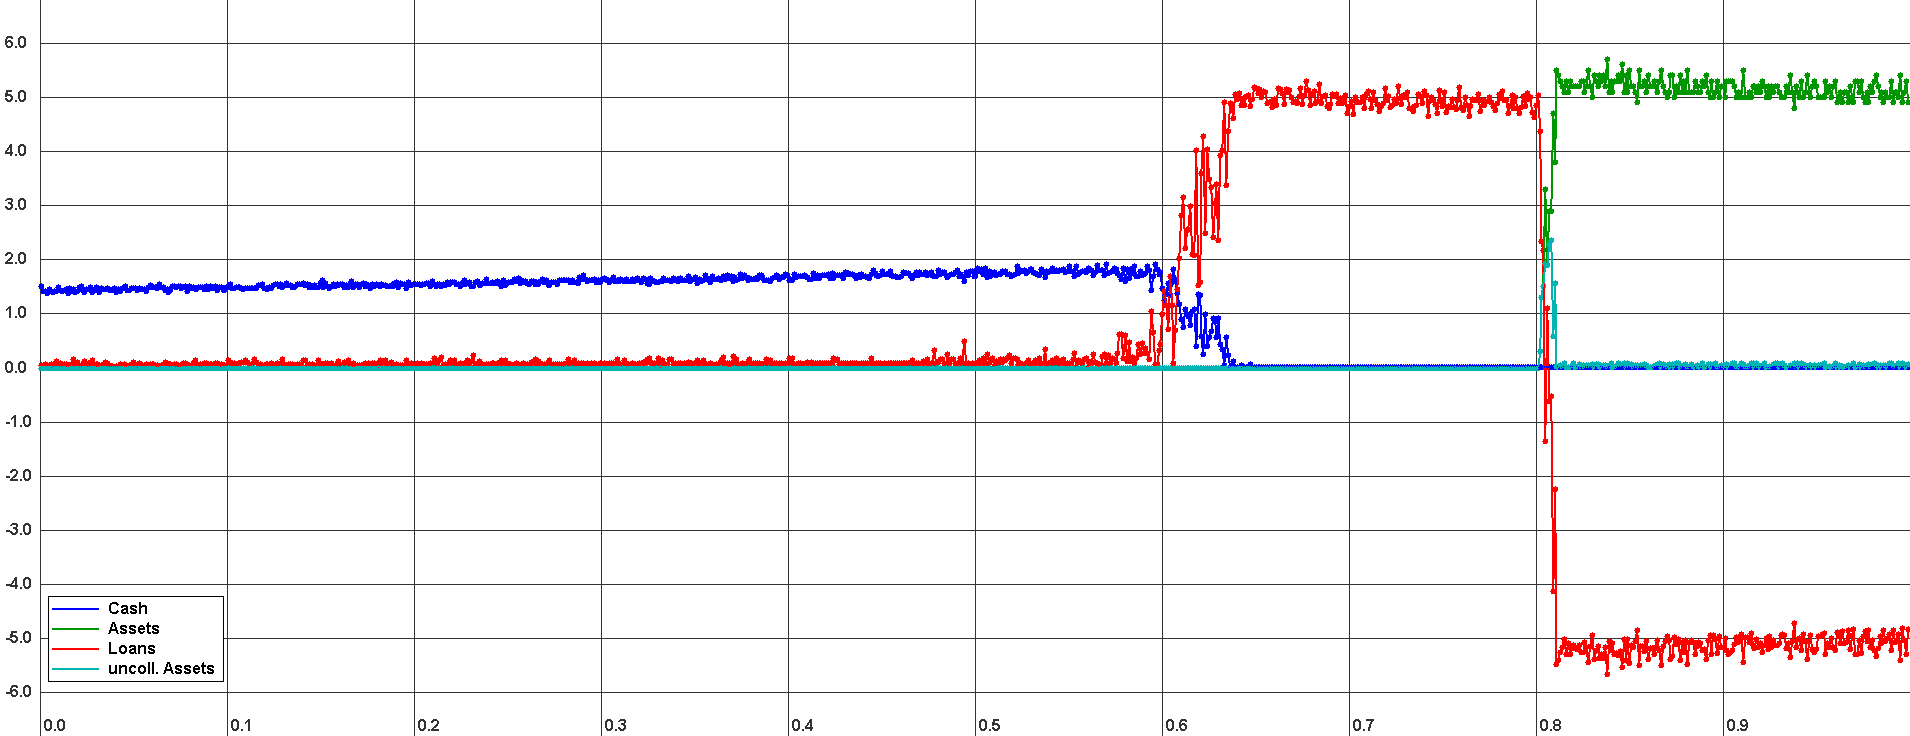
\includegraphics[width=1.0\textwidth, angle=0]{FULLYCONNECTED_1000_NOCOLLATERALMARKET_SINGLE.png}
	\caption{Thesis-Implementation wealth-distribution of Fully-Connected topology after single run}
	\label{fig1}
\end{figure}

\begin{figure}[!htbp]
	\centering
  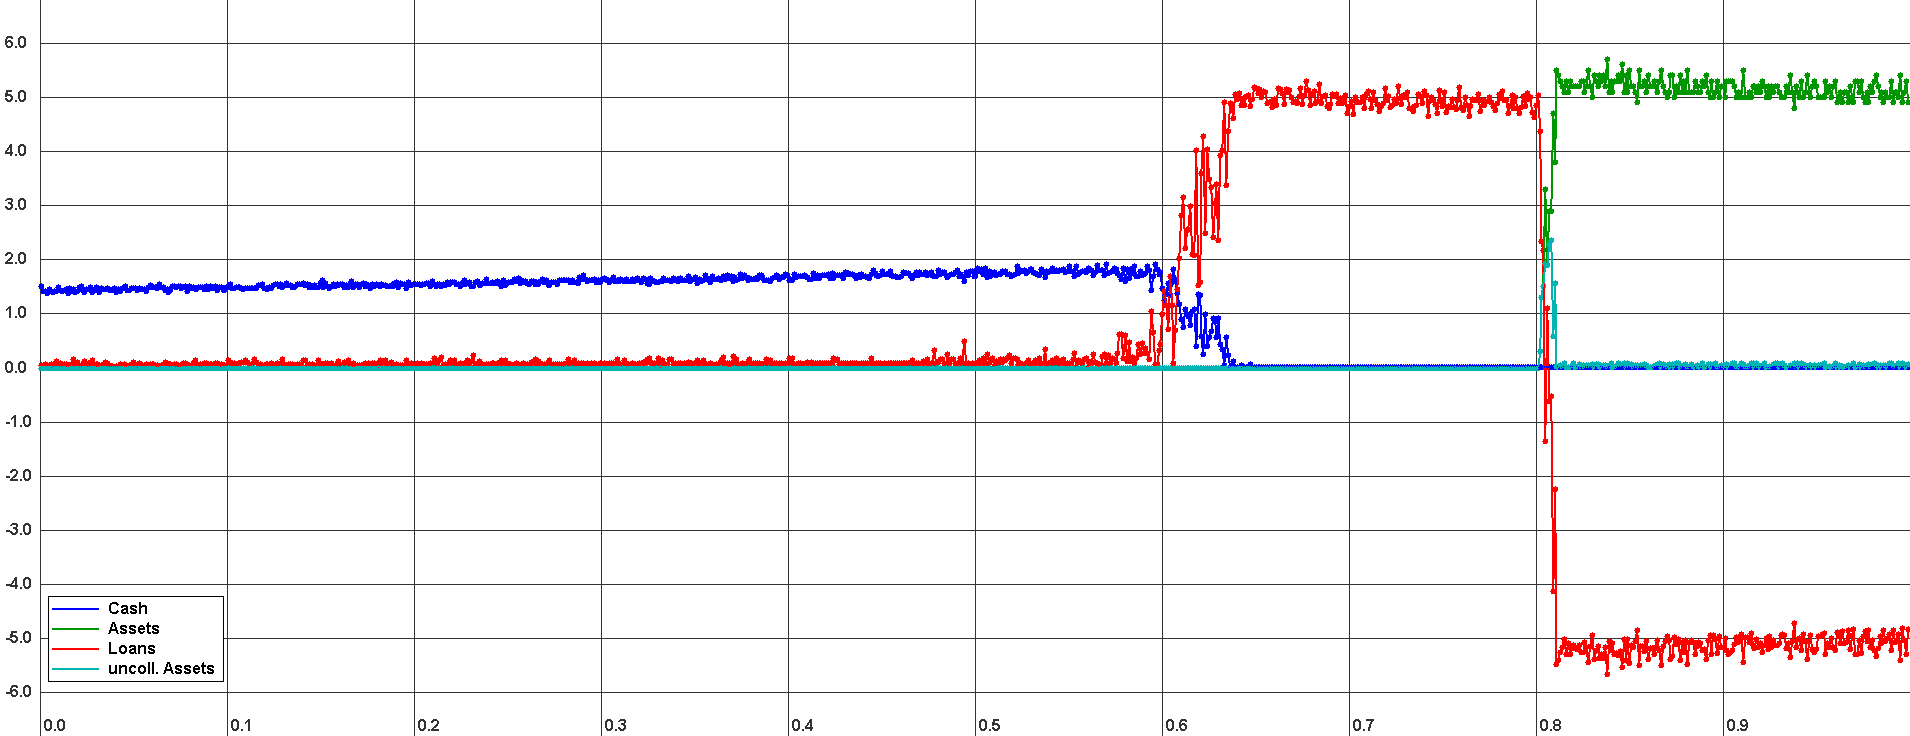
\includegraphics[width=1.0\textwidth, angle=0]{FULLYCONNECTED_1000_NOCOLLATERALMARKET_SINGLE.png}
	\caption{Thesis-Implementation wealth-distribution of Fully-Connected topology after 50 replications}
	\label{fig1}
\end{figure}

\begin{table}[h]
	\centering
	\caption{Equilibrium of thesis-implementation}
	\begin{tabular} { l c r }
		\hline
		Asset-Price & TODO (TODO) \\
		Loan-Price & TODO (TODO) \\
		i0 (Marginal Buyer) & TODO (TODO) \\
		i1 (Marginal Seller) & TODO (TODO) \\
		Pessimist Wealth & TODO (TODO) \\
		Medianist Wealth & TODO (TODO) \\
		Optimist Wealth & TODO (TODO) \\
		\hline
	\end{tabular}
\end{table}



\begin{table}[h]
	\centering
	\caption{Performance of thesis-implementation with 1000 Agents and 0.5 Bond}
	\begin{tabular} { l c r }
		\hline
		Successful TX & TODO (TODO) \\
		Total TX & TODO (TODO) \\
		Failed TX & TODO (TODO) \\
		\hline
	\end{tabular}
\end{table}

\begin{table}[h]
	\centering
	\caption{Equilibrium in \cite{Breuer2015} with 1000 Agents and 0.5 Bond }
	\begin{tabular} { l c r }
		\hline
		Asset-Price p & 0.716 \\
		Loan-Price q & 0.375 \\
		Marginal Buyer i0 & 0.583 \\
		Marginal Seller i1 & 0.801 \\
		Pessimist Wealth & 1.716 \\
		Medianist Wealth & 4.578 \\
		Optimist Wealth & 5.032 \\
		\hline
	\end{tabular}
\end{table}

// TODO: difference to breuer 
// TODO: difference to theoretical equilibrium

\section{Experiments configuration}
In the following experiments 100 Agents were used, all markets were enabled, the bond-type 0.5 was selected and if replications were used always 50 were run.
As Termination-Mode "Failed successive Transactions" is selected with the number of failed transactions in a row is 1000. Note that if trading is not possible any more before these 1000 failed transactions have been reached, the simulation is halted and thus it is possible that it terminates earlier.

100 agents were chosen because \cite{Breuer2015} showed that equilibrium can be reached already with 30 agents so this was the minimum number of agents to start with. For a finer "resolution" of the visual results 100 were chosen also because its a good match between too much processing power required and nice visual results.
The 0.5 Bond was selected because its a risky one and only when a risky bond is traded then will this equilibirum show up as for unrisky bonds with Facevalue <= 0.2 the results are indifferent.
Obviously the whole simulation-process is a random-process with an equilibrium (different for each topology) as the fixed-point solution thus one needs replications to reduce noise. The number of 50 Replications was chosen because its a good match between run-time duration and overall reduction of noise - increasing the number e.g. to 100 or 200 would not result in much better results but would need much longer to run. All facts can be seen and derived when using 50 replications.

Theoretical equilibrium for i0, i1, asset price and loan price can be calculated and are as follows:

\begin{table}[h]
	\centering
	\caption{Theoretical Equilibrium for 100 Agents}
	\begin{tabular} { l c r }
		\hline
		Asset-Price p & 0.716 \\
		Loan-Price q & 0.384 \\
		Marginal Buyer i0 & 0.584 \\
		Marginal Seller i1 & 0.801 \\
		\hline
	\end{tabular}
\end{table}





\section{Fully-Connected Topology}


It is also a point-of-reference for the other experiments as this fully-connected topology gives a good point of visual information which can be applied to the other topologies to give a visual clue whether they could have actually reached the equilibrium.

TODO: is a single-run really necessary? seems to be necessary only for ascending-connected 

\begin{figure}[!htbp]
	\centering
  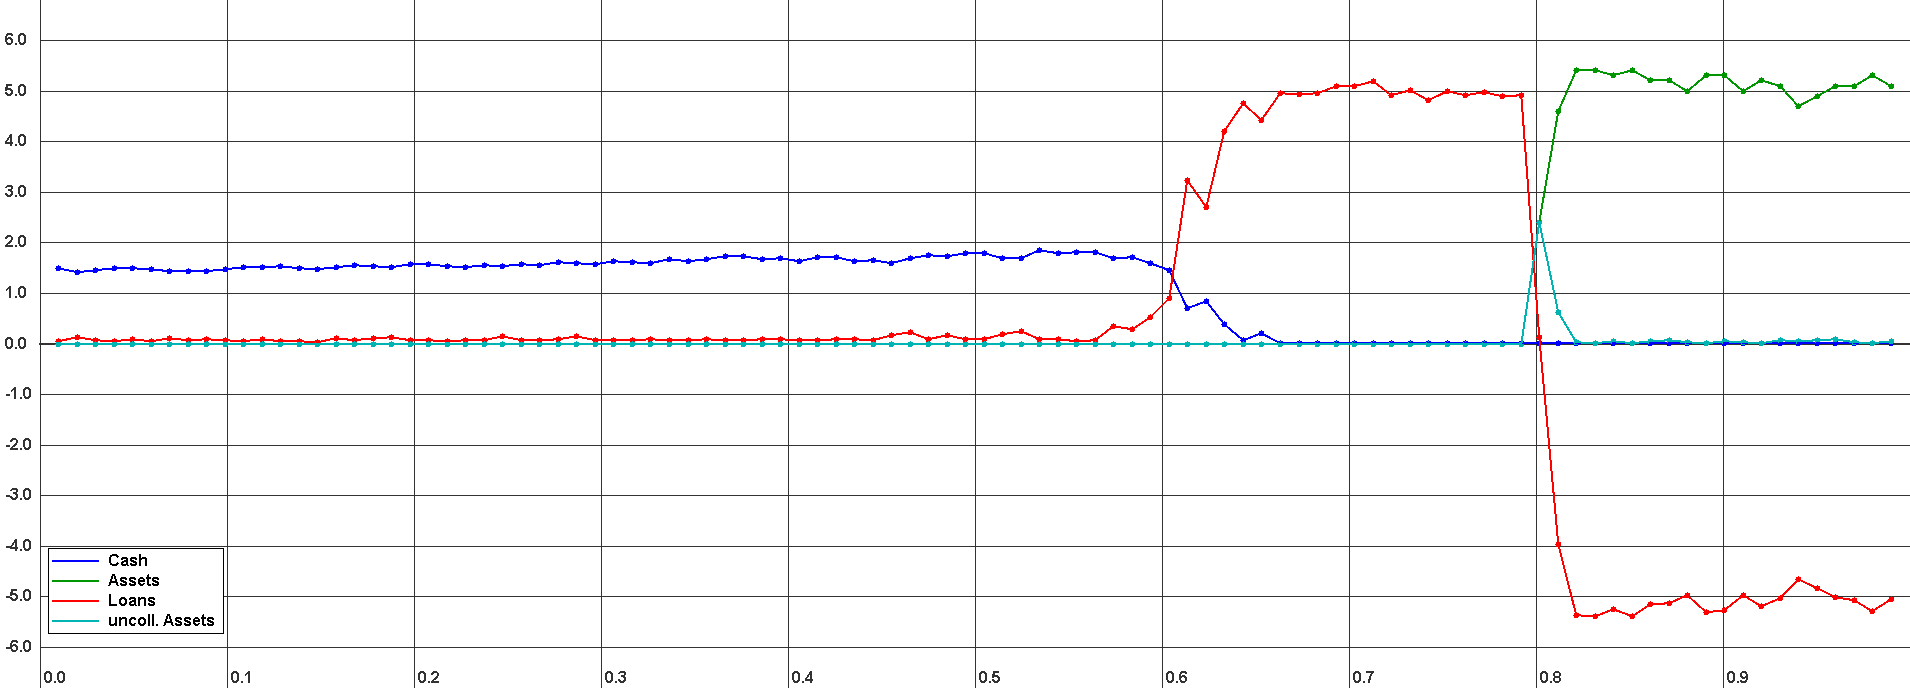
\includegraphics[width=1.0\textwidth, angle=0]{FULLYCONNECTED_100_NOCOLLATERALMARKET_SINGLE.png}
	\caption{Fully-Connected wealth-distribution after single run}
	\label{fig1}
\end{figure}

\begin{figure}[!htbp]
	\centering
  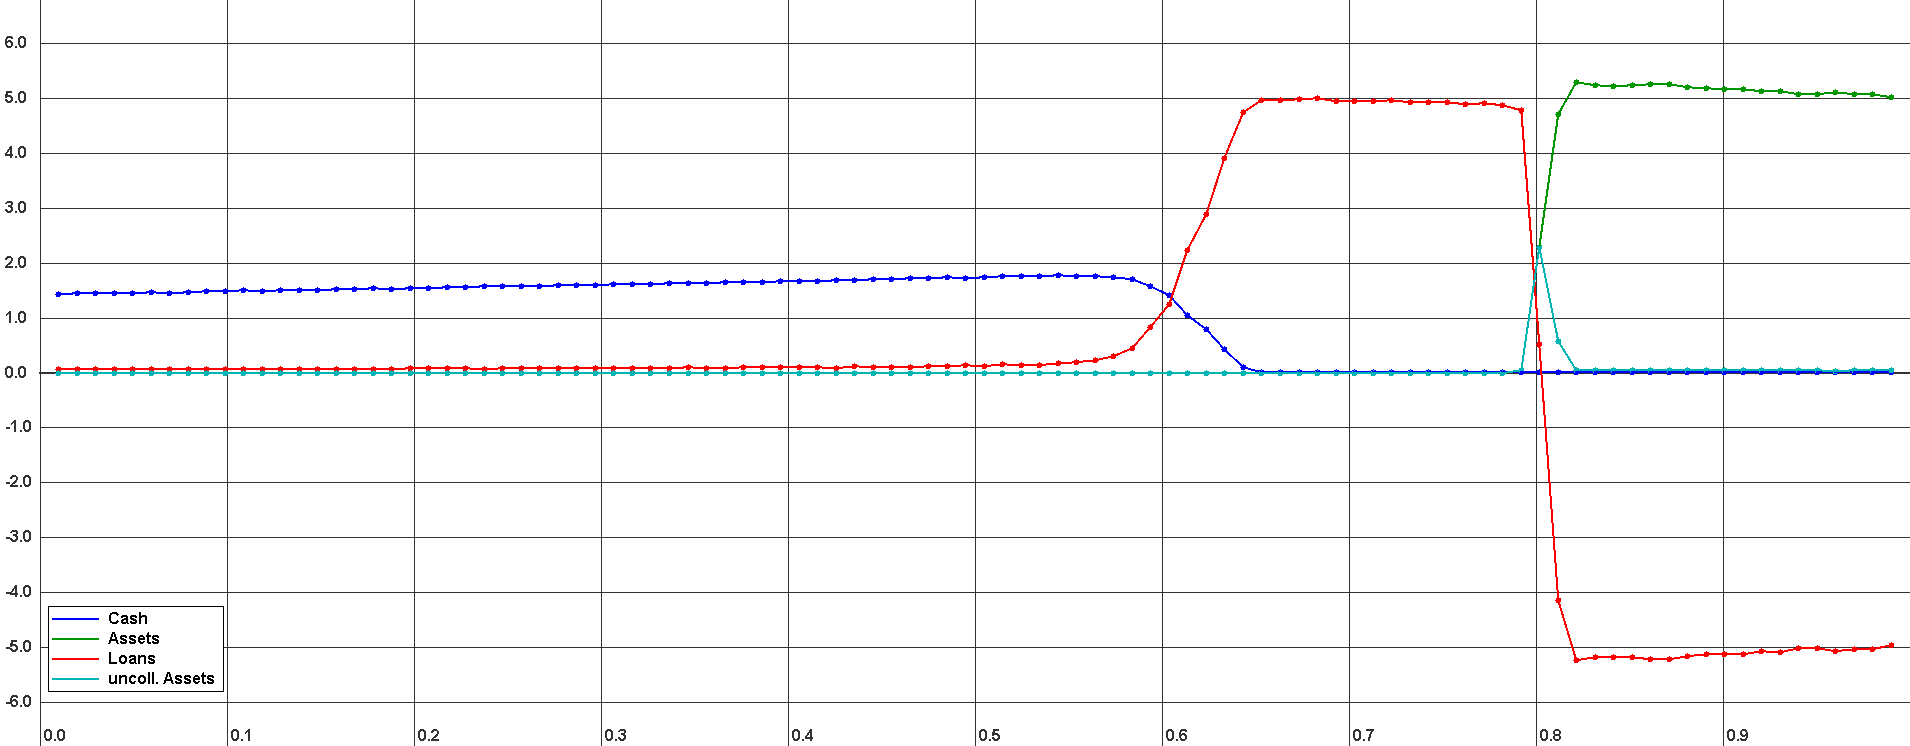
\includegraphics[width=1.0\textwidth, angle=0]{FULLYCONNECTED_100_NOCOLLATERALMARKET_REPL.png}
	\caption{Fully-Connected wealth-distribution after 50 replications}
	\label{fig1}
\end{figure}

\begin{table}[h]
	\caption{Equilibrium for 100 Agents}
	\centering
	\begin{tabular} { l c r }
		\hline
		Asset-Price & 0.689 (0.010) \\
		Loan-Price & 0.384 (0.004) \\
		i0 (Marginal Buyer) & 0.603 (0.007) \\
		i1 (Marginal Seller) & 0.803 (0.003) \\
		Pessimist Wealth & 1.597 (0.015) \\
		Medianist Wealth & 4.565 (0.113) \\
		Optimist Wealth & 5.021 (0.064) \\
		\hline
	\end{tabular}
\end{table} 

\begin{table}[h]
	\caption{Performance of 100 Agents}
	\centering
	\begin{tabular} { l c r }
		\hline
		Successful TX & 1916.14 (31.42) \\
		Total TX & 6364.8 (1679.21) \\
		Failed TX & 4448.66 (1668.93) \\
		\hline
	\end{tabular}
\end{table}

\subsection{Half-Fully Connected}
\begin{figure}[!htbp]
	\centering
  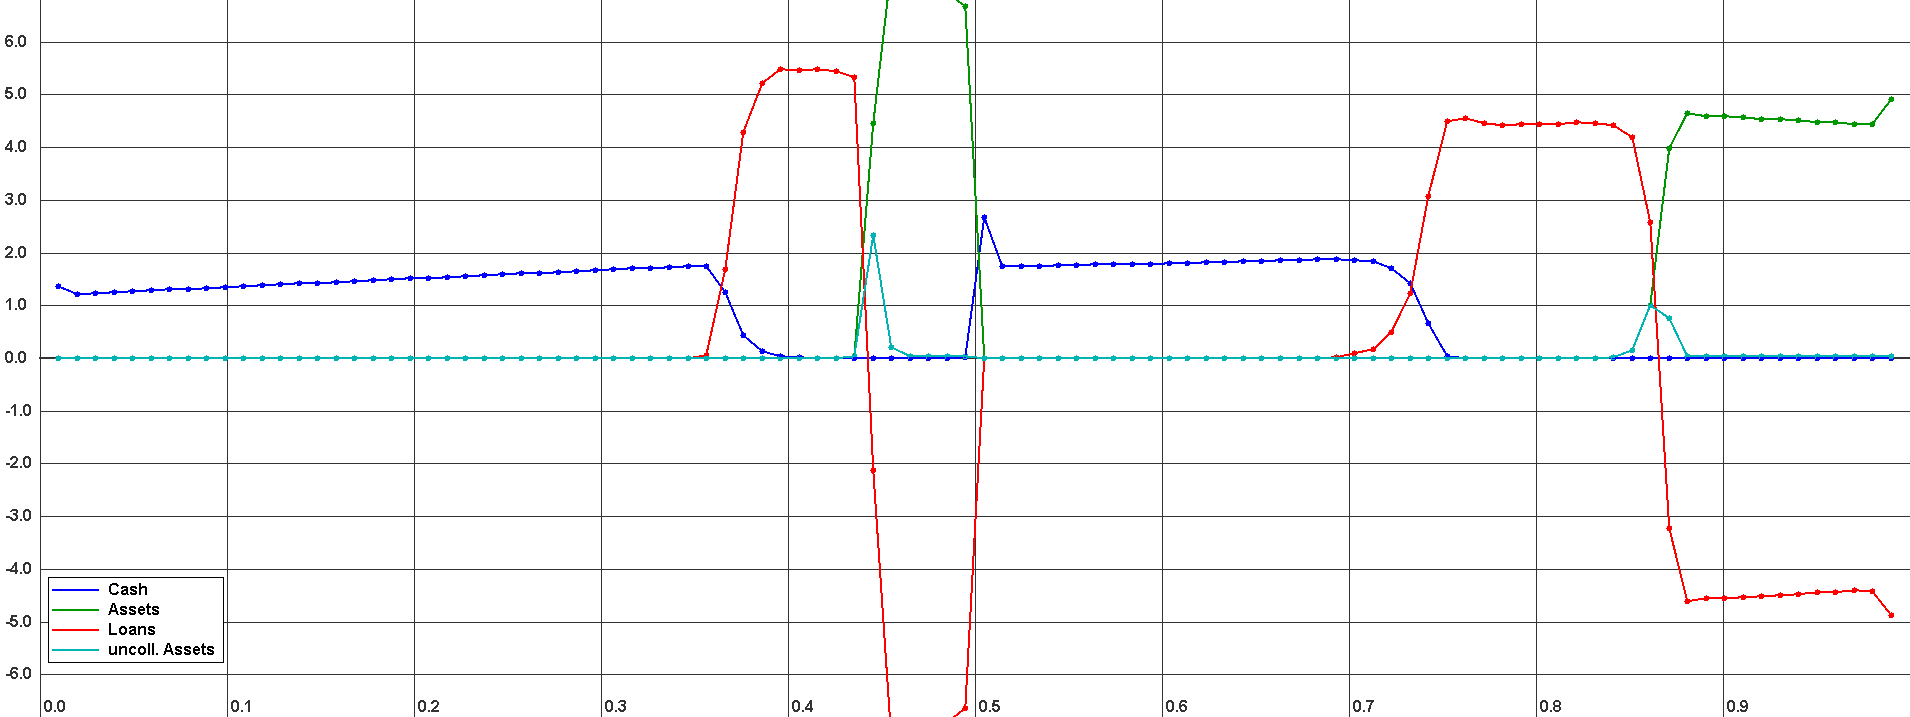
\includegraphics[width=1.0\textwidth, angle=0]{HALFFULLYCONNECTED_100_NOCOLLATERALMARKET_REPL.png}
	\caption{Half-Fully connected wealth-distribution after 50 replications}
	\label{fig1}
\end{figure}

\begin{table}[!htbp]
	\caption{Half-Fully connected equilibrium for 100 Agents}
	\centering
	\begin{tabular} { l c r }
		\hline
		Asset-Price & 0.651 (0.027) \\
		Loan-Price & 0.362 (0.013) \\
		i0 (Marginal Buyer) & 0.640 (0.015) \\
		i1 (Marginal Seller) & 0.833 (0.09) \\
		Pessimist Wealth & 1.22 (0.096) \\
		Medianist Wealth & 2.258 (0.409) \\
		Optimist Wealth & 4.526 (0.071) \\
		\hline
	\end{tabular}
\end{table} 

\begin{table}[!htbp]
	\caption{Ascending-Connected 30 regular short-cuts performance of 100 Agents}
	\centering
	\begin{tabular} { l c r }
		\hline
		Successful TX & 14,218.9 (4621.74) \\
		Total TX & 15,253.02 (4633.44) \\
		Failed TX & 1034.12 (22.99) \\
		\hline
	\end{tabular}
\end{table}

\section{Ascending-Connected Topologies} 

\subsection{Ascending-Connected}
\begin{figure}[!htbp]
	\centering
  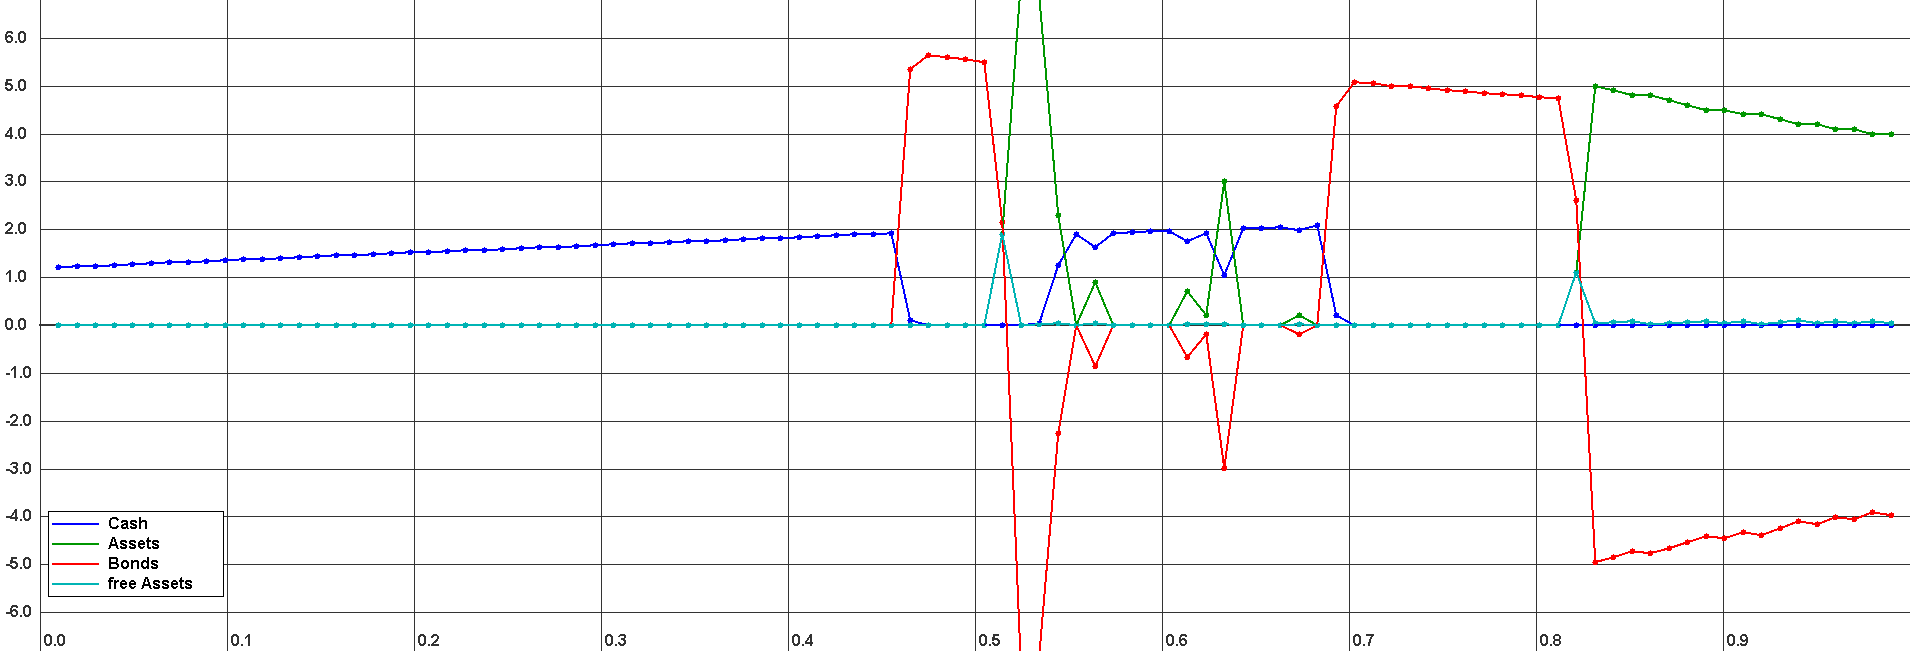
\includegraphics[width=1.0\textwidth, angle=0]{ASCENDINGCONNECTED_100_NOCOLLATERALMARKET_SINGLE.png}
	\caption{Ascending-Connected wealth-distribution after single run}
	\label{fig1}
\end{figure}

\begin{figure}[!htbp]
	\centering
  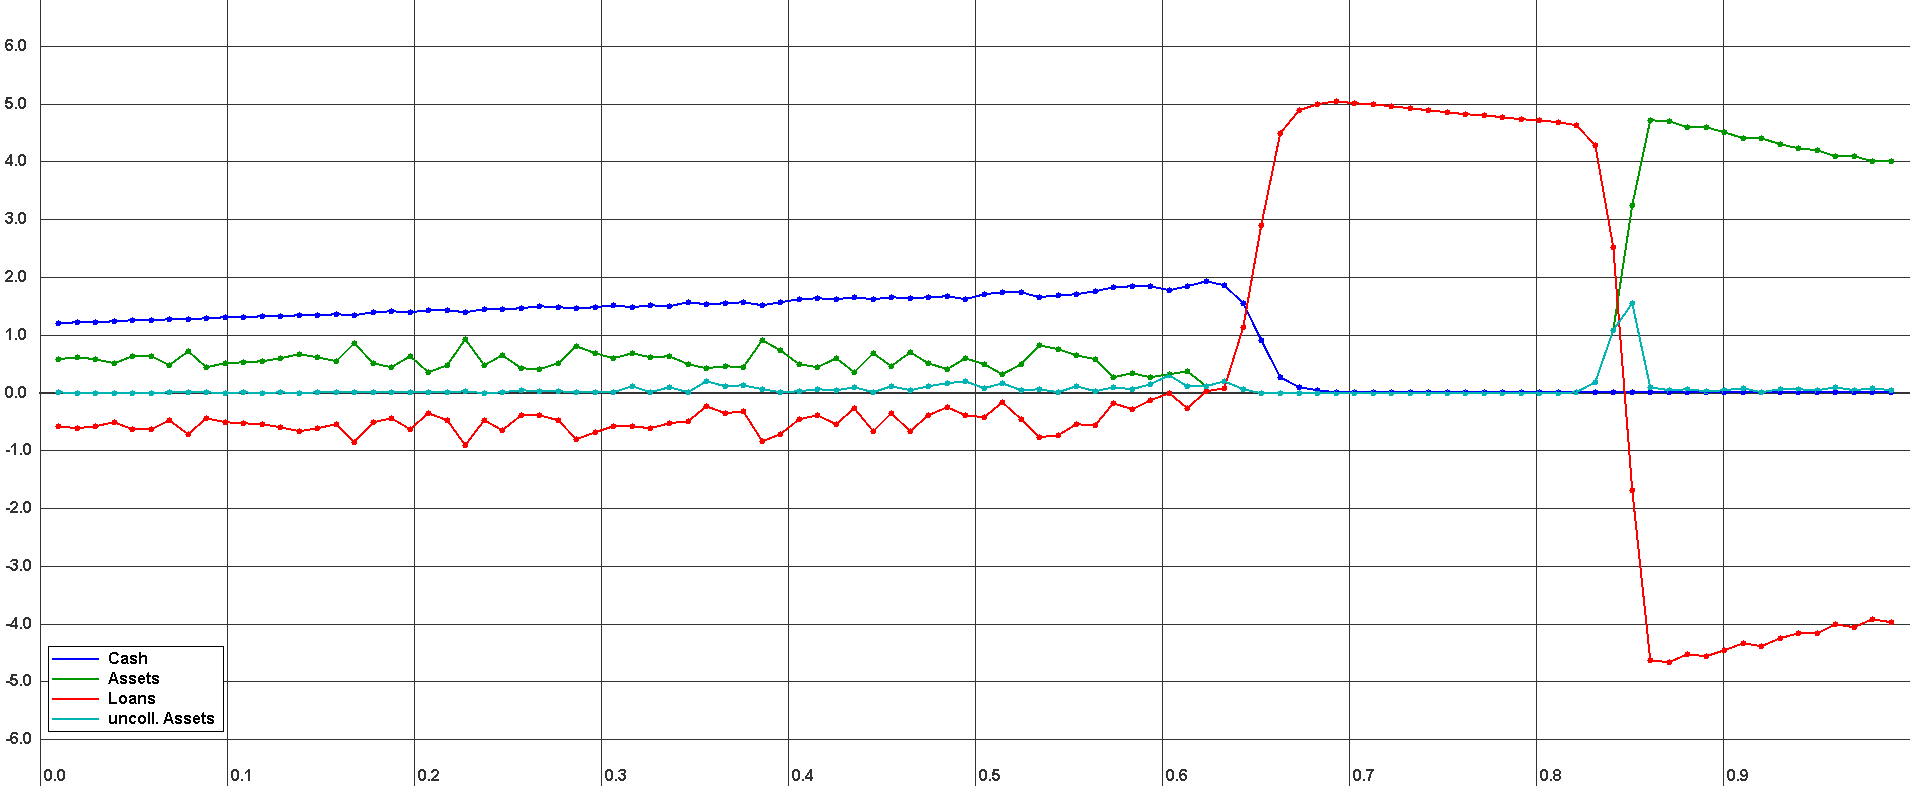
\includegraphics[width=1.0\textwidth, angle=0]{ASCENDINGCONNECTED_100_NOCOLLATERALMARKET_REPL.png}
	\caption{Ascending-Connected wealth-distribution after 50 replications}
	\label{fig1}
\end{figure}

\begin{table}[h]
	\caption{Ascending-Connected equilibrium for 100 Agents}
	\centering
	\begin{tabular} { l c r }
		\hline
		Asset-Price & 0.711 (0.016) \\
		Loan-Price & 0.391 (0.005) \\
		i0 (Marginal Buyer) & 0.646(0.012) \\
		i1 (Marginal Seller) & 0.850 (0.008) \\
		Pessimist Wealth & 1.166 (0.072) \\
		Medianist Wealth & 1.869 (0.243) \\
		Optimist Wealth & 4.307 (0.070) \\
		\hline
	\end{tabular}
\end{table} 

\begin{table}[h]
	\caption{Ascending-Connected performance of 100 Agents}
	\centering
	\begin{tabular} { l c r }
		\hline
		Successful TX & 36,940.96 (1948.69) \\
		Total TX & 38,117.04 (1934.06) \\
		Failed TX & 1176.08 (98.01) \\
		\hline
	\end{tabular}
\end{table}

TODO: move to interpretation: As can be clearly seen the equilibrium is fundamentally different than the fully-connected one and thus the hypothesis is not satisfied.

\subsection{Ascending-Connected Importance Sampling}
\begin{figure}[!htbp]
	\centering
  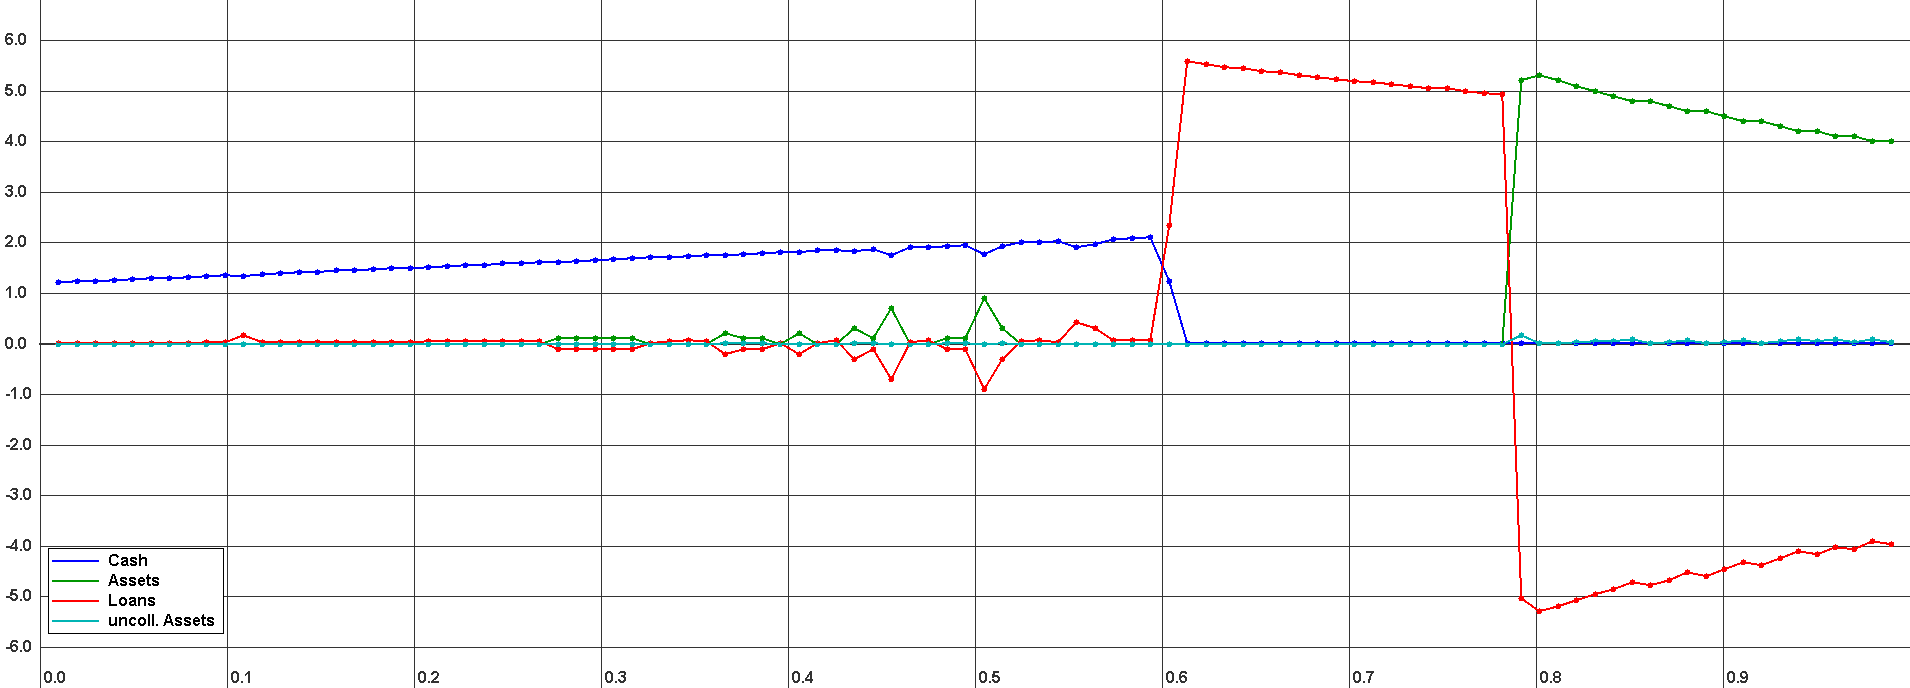
\includegraphics[width=1.0\textwidth, angle=0]{ASCENDINGCONNECTED_IS_100_NOCOLLATERALMARKET_SINGLE.png}
	\caption{Ascending-Connected Importance Sampling wealth-distribution after single run}
	\label{fig1}
\end{figure}

\begin{figure}[!htbp]
	\centering
  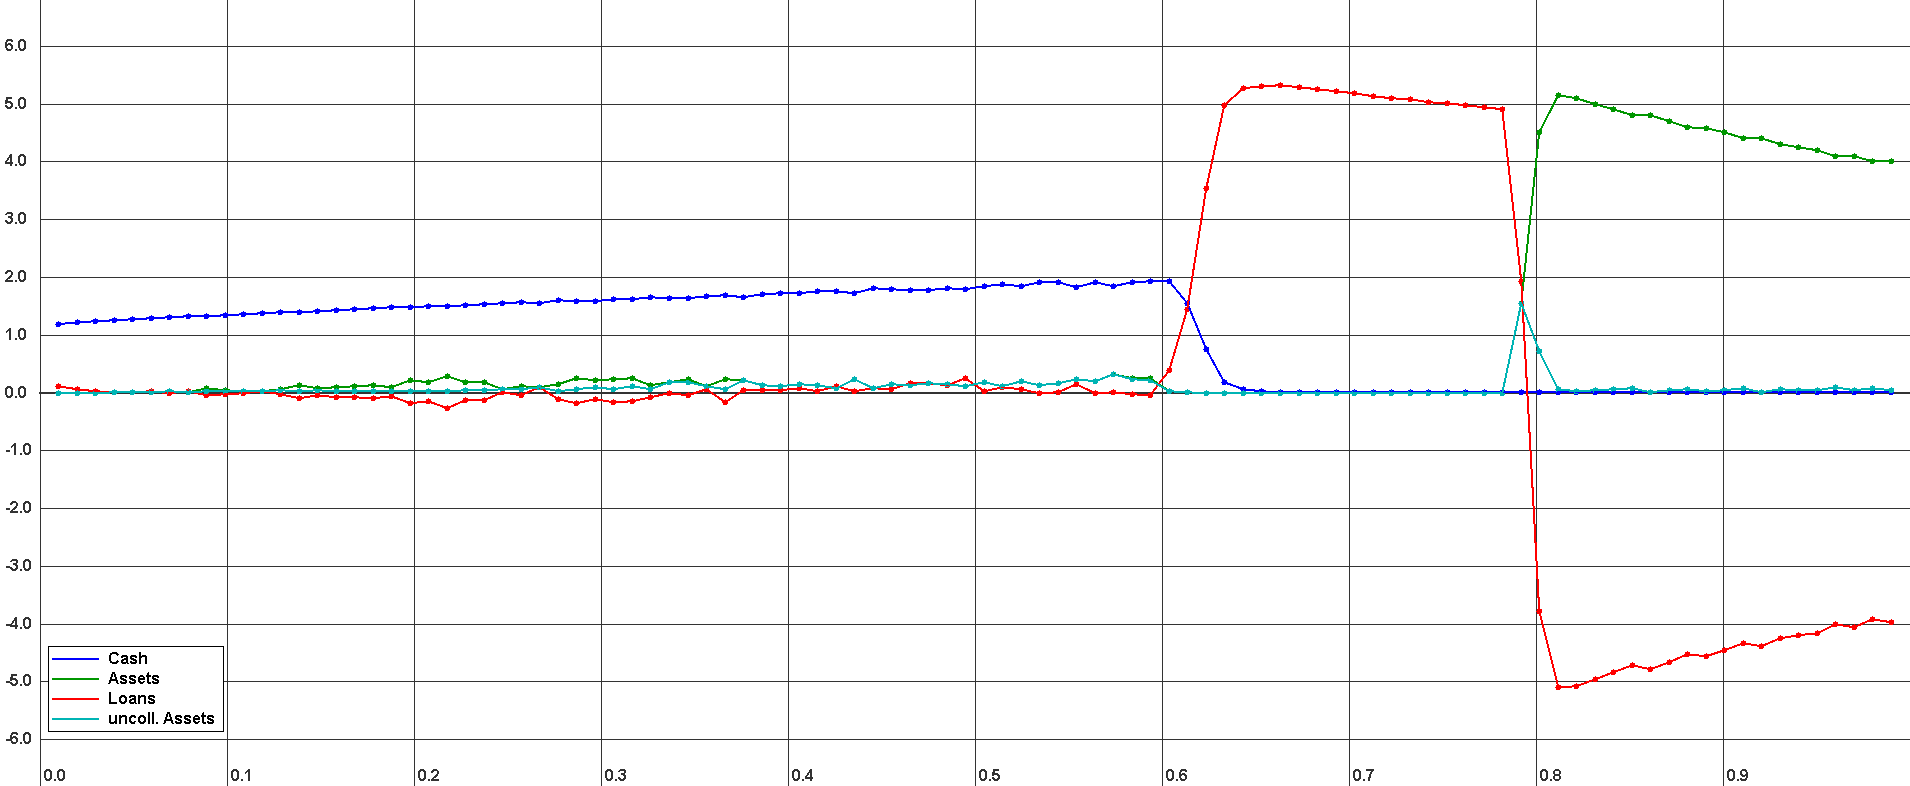
\includegraphics[width=1.0\textwidth, angle=0]{ASCENDINGCONNECTED_IS_100_NOCOLLATERALMARKET_REPL.png}
	\caption{Ascending-Connected Importance Sampling wealth-distribution after 50 replications}
	\label{fig1}
\end{figure}

\begin{table}[h]
	\caption{Ascending-Connected Importance Sampling equilibrium for 100 Agents}
	\centering
	\begin{tabular} { l c r }
		\hline
		Asset-Price & 0.691 (0.009) \\
		Loan-Price & 0.383 (0.004) \\
		i0 (Marginal Buyer) & 0.614 (0.009) \\
		i1 (Marginal Seller) & 0.799 (0.006) \\
		Pessimist Wealth & 1.497 (0.072) \\
		Medianist Wealth & 3.934 (0.505) \\
		Optimist Wealth & 4.519 (0.051) \\
		\hline
	\end{tabular}
\end{table} 

\begin{table}[h]
	\caption{Ascending-Connected Importance Sampling performance of 100 Agents}
	\centering
	\begin{tabular} { l c r }
		\hline
		Successful TX & 49,881.6 (1733.33) \\
		Total TX & 49,882.6 (1733.33) \\
		Failed TX & 1.0 (0.00) \\
		\hline
	\end{tabular}
\end{table}

Note that in this case the matching-probabilities are such that upon the first failed transaction the equilibrium has reached as no agent can trade with each other anymore which results in just on single failed transaction.

TODO: move to interpretation: As can be clearly seen the equilibrium is fundamentally different than the fully-connected one and thus the hypothesis is not satisfied.

\subsection{Ascending-Connected 5 full Short-cuts }
\begin{figure}[!htbp]
	\centering
  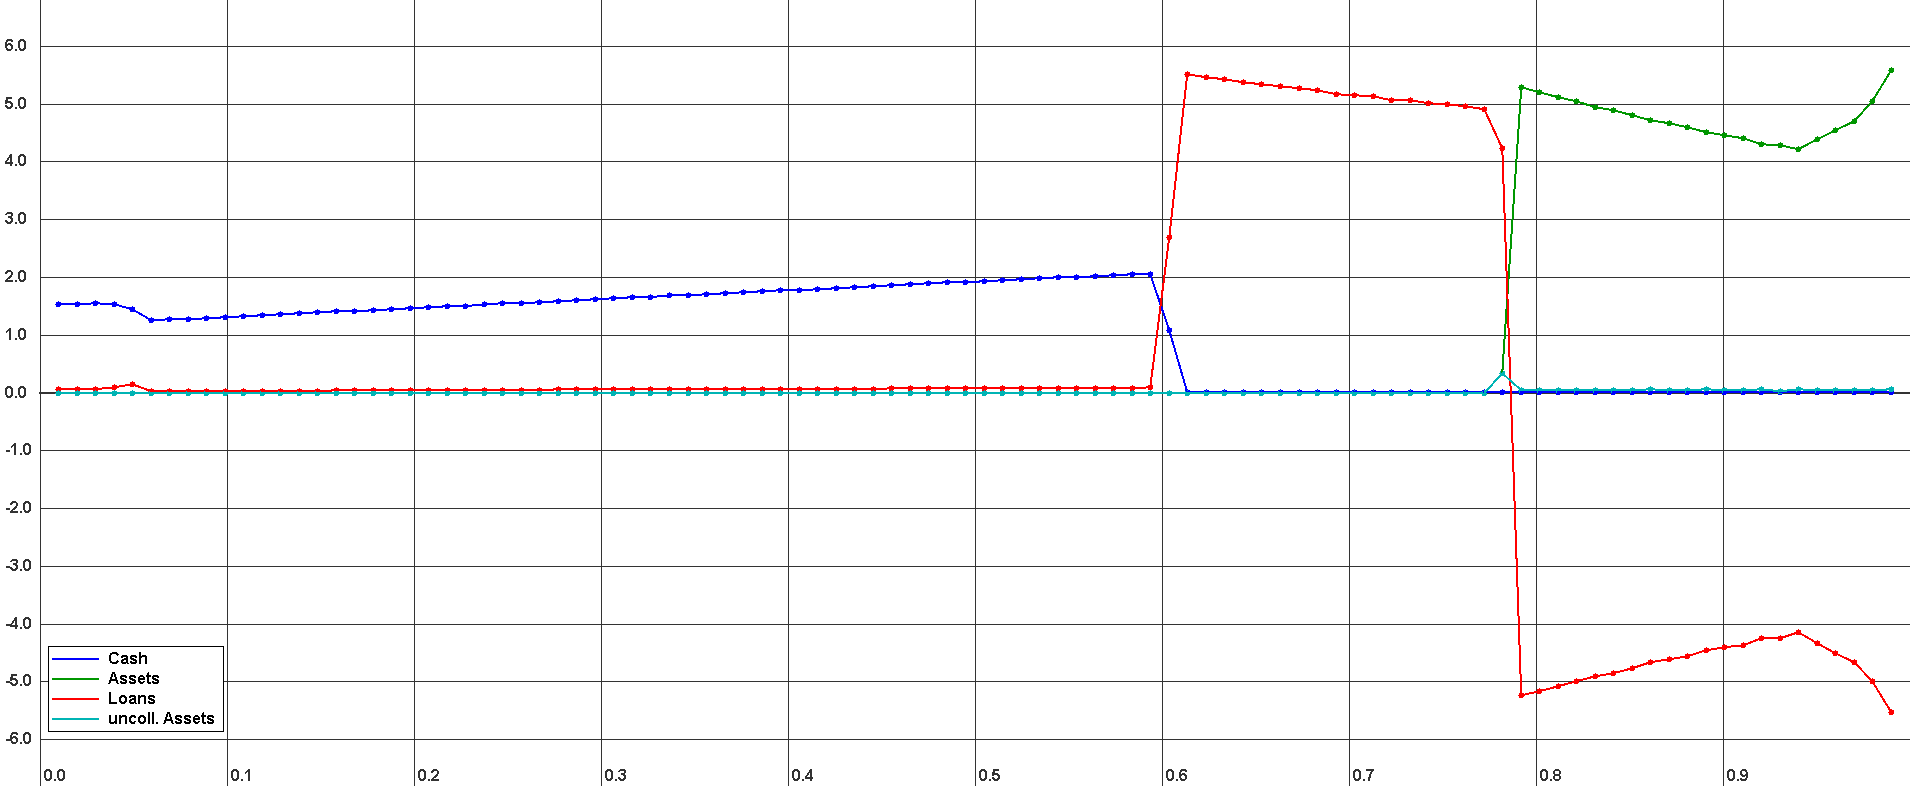
\includegraphics[width=1.0\textwidth, angle=0]{ASCENDINGCONNECTED_5FullSC_100_NOCOLLATERALMARKET_REPL.png}
	\caption{Ascending-Connected 5 full short-cuts wealth-distribution after 50 replications}
	\label{fig1}
\end{figure}

\begin{table}[h]
	\caption{Ascending-Connected 5 full short-cuts equilibrium for 100 Agents}
	\centering
	\begin{tabular} { l c r }
		\hline
		Asset-Price & 0.656 (0.019) \\
		Loan-Price & 0.371 (0.003) \\
		i0 (Marginal Buyer) & 0.594 (0.0) \\
		i1 (Marginal Seller) & 0.792 (0.0) \\
		Pessimist Wealth & 1.649 (0.002) \\
		Medianist Wealth & 5.013 (0.018) \\
		Optimist Wealth & 4.746 (0.011) \\
		\hline
	\end{tabular}
\end{table} 

\begin{table}[h]
	\caption{Ascending-Connected 5 full short-cuts performance of 100 Agents}
	\centering
	\begin{tabular} { l c r }
		\hline
		Successful TX & 16,971.34 (228.0) \\
		Total TX & 17,998.26 (225.23) \\
		Failed TX & 1026.92 (22.68) \\
		\hline
	\end{tabular}
\end{table}

TODO: move to interpretation: As can be clearly seen 5 full shortcuts seem to be already enough to solve the inefficiencies seen in Ascending-Connected with/without Importance Sampling.

\subsection{Ascending-Connected 15 full Short-cuts }
\begin{figure}[!htbp]
	\centering
  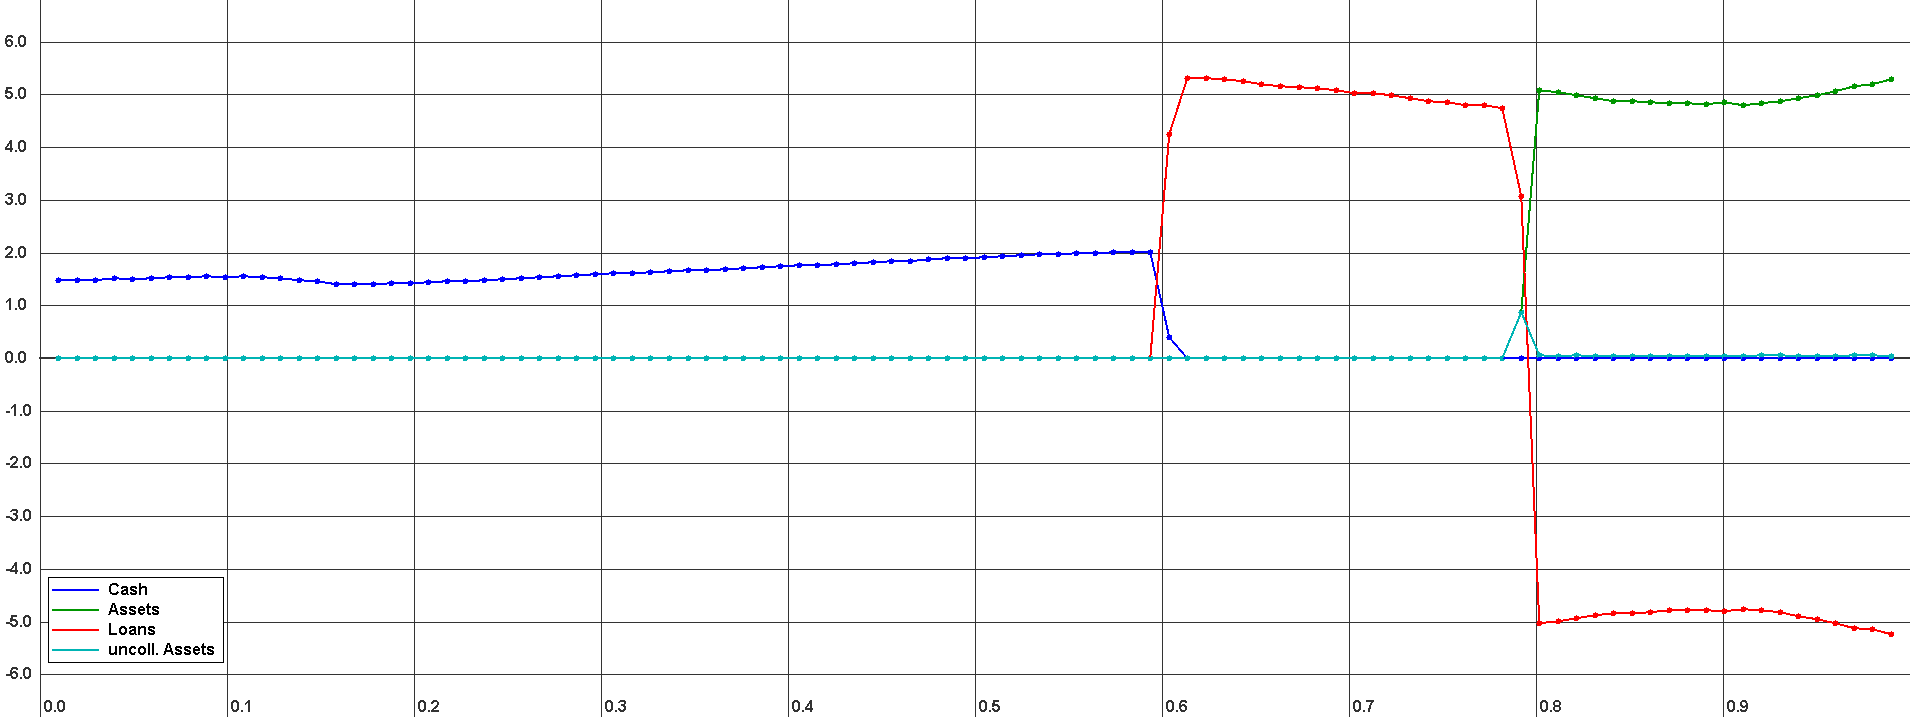
\includegraphics[width=1.0\textwidth, angle=0]{ASCENDINGCONNECTED_15FullSC_100_NOCOLLATERALMARKET_REPL.png}
	\caption{Ascending-Connected 15 full short-cuts wealth-distribution after 50 replications}
	\label{fig1}
\end{figure}

\begin{table}[h]
	\caption{Ascending-Connected 15 full short-cuts equilibrium for 100 Agents}
	\centering
	\begin{tabular} { l c r }
		\hline
		Asset-Price & 0.658 (0.024) \\
		Loan-Price & 0.366 (0.009) \\
		i0 (Marginal Buyer) & 0.601 (0.004) \\
		i1 (Marginal Seller) & 0.802 (0.0) \\
		Pessimist Wealth & 1.649 (0.004) \\
		Medianist Wealth & 4.811 (0.092) \\
		Optimist Wealth & 4.957 (0.021) \\
		\hline
	\end{tabular}
\end{table} 

\begin{table}[!htbp]
	\caption{Ascending-Connected 15 full short-cuts performance of 100 Agents}
	\centering
	\begin{tabular} { l c r }
		\hline
		Successful TX & 4498.08 (58.67) \\
		Total TX & 5522.860 (64.72) \\
		Failed TX & 1024.78 (17.3) \\
		\hline
	\end{tabular}
\end{table}

\subsection{Ascending-Connected 30 full Short-cuts }
\begin{figure}[!htbp]
	\centering
  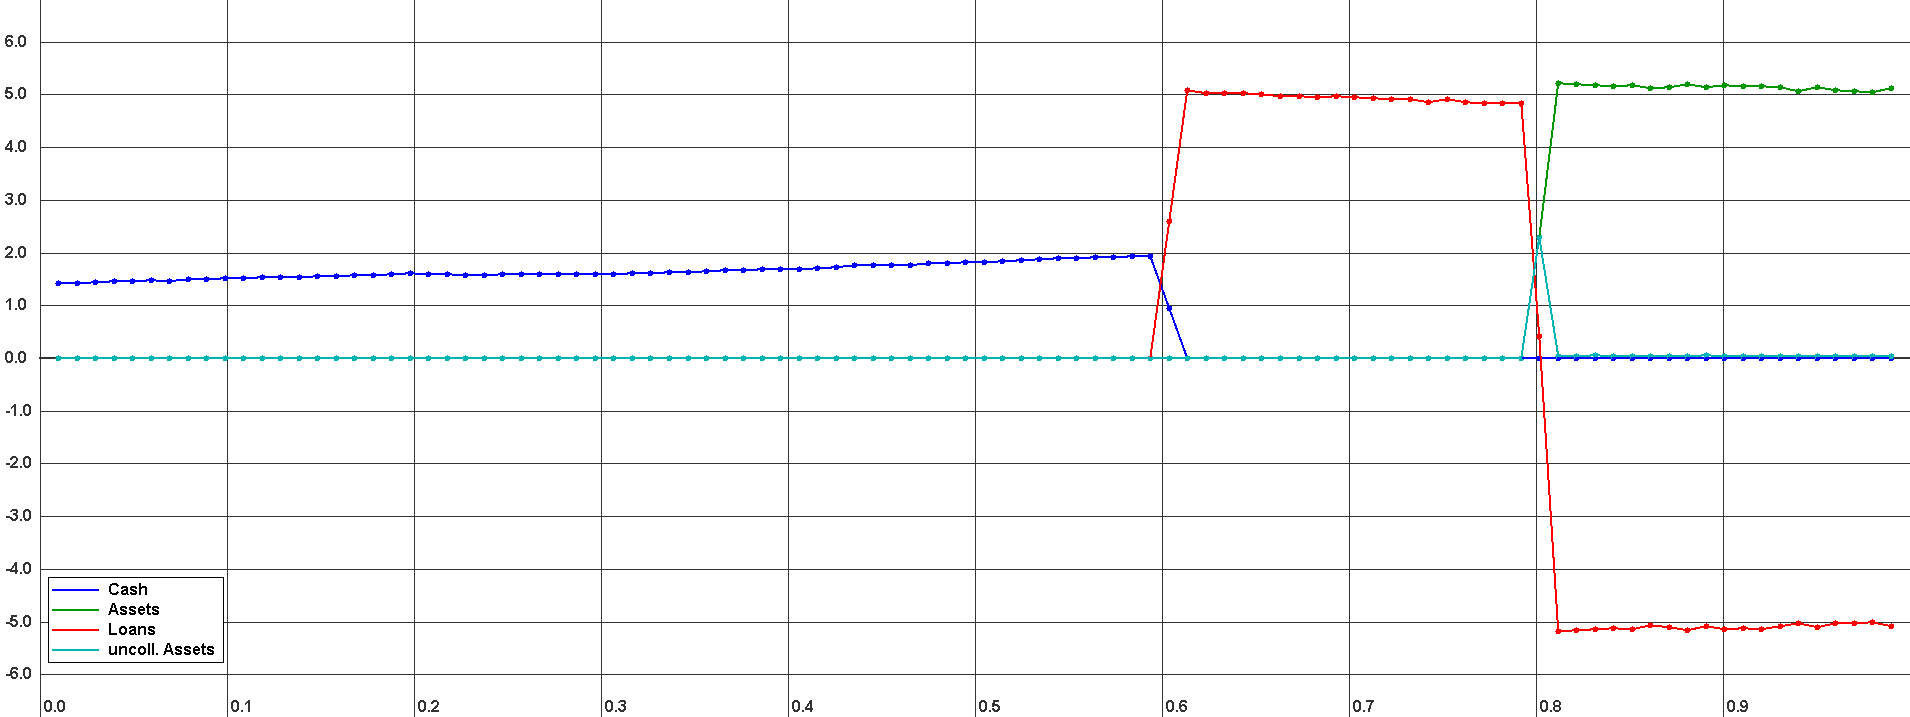
\includegraphics[width=1.0\textwidth, angle=0]{ASCENDINGCONNECTED_30FullSC_100_NOCOLLATERALMARKET_REPL.png}
	\caption{Ascending-Connected 30 full short-cuts wealth-distribution after 50 replications}
	\label{fig1}
\end{figure}

\begin{table}[!htbp]
	\caption{Ascending-Connected 30 full short-cuts equilibrium for 100 Agents}
	\centering
	\begin{tabular} { l c r }
		\hline
		Asset-Price & 0.681 (0.012) \\
		Loan-Price & 0.378 (0.006) \\
		i0 (Marginal Buyer) & 0.603 (0.006) \\
		i1 (Marginal Seller) & 0.802 (0.1) \\
		Pessimist Wealth & 1.649 (0.009) \\
		Medianist Wealth & 4.702 (0.112) \\
		Optimist Wealth & 5.004 (0.025) \\
		\hline
	\end{tabular}
\end{table} 

\begin{table}[!htbp]
	\caption{Ascending-Connected 30 full short-cuts performance of 100 Agents}
	\centering
	\begin{tabular} { l c r }
		\hline
		Successful TX & 2211.08 (35.88) \\
		Total TX & 3225.76 (40.18) \\
		Failed TX & 1014.68 (10.55) \\
		\hline
	\end{tabular}
\end{table}


\subsection{Ascending-Connected 5 regular Short-cuts }
\begin{figure}[!htbp]
	\centering
  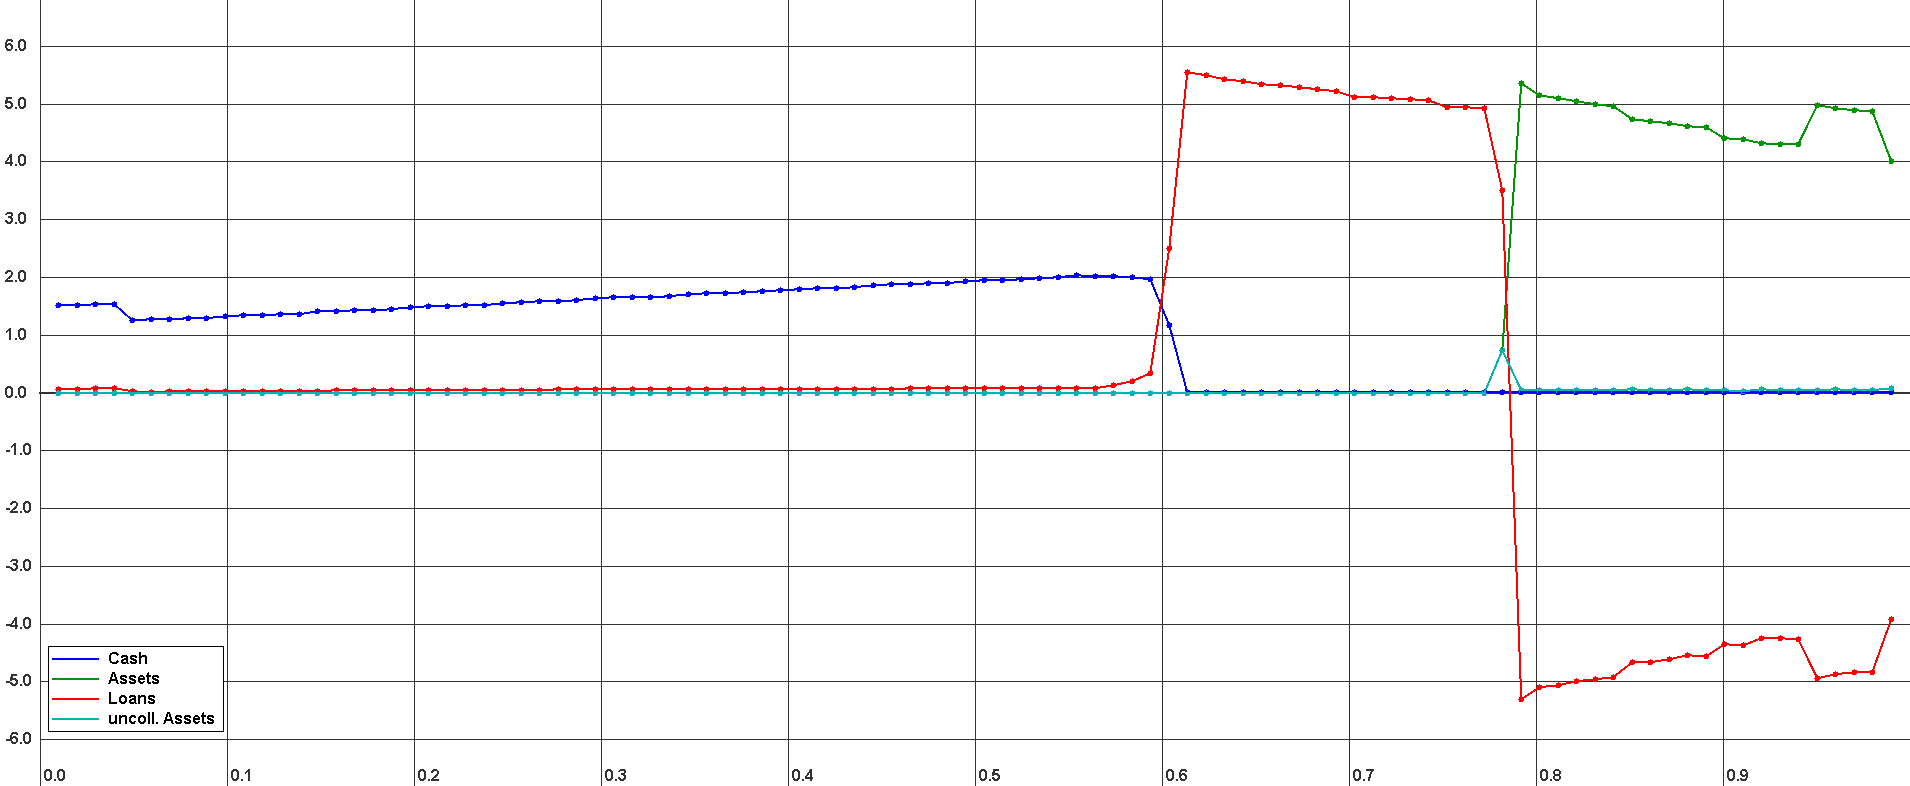
\includegraphics[width=1.0\textwidth, angle=0]{ASCENDINGCONNECTED_5RegSC_100_NOCOLLATERALMARKET_REPL.png}
	\caption{Ascending-Connected 5 regular short-cuts wealth-distribution after 50 replications}
	\label{fig1}
\end{figure}

\begin{table}[!htbp]
	\caption{Ascending-Connected 5 regular short-cuts equilibrium for 100 Agents}
	\centering
	\begin{tabular} { l c r }
		\hline
		Asset-Price & 0.665 (0.016) \\
		Loan-Price & 0.364 (0.007) \\
		i0 (Marginal Buyer) & 0.595 (0.003) \\
		i1 (Marginal Seller) & 0.792 (0.0) \\
		Pessimist Wealth & 1.649 (0.003) \\
		Medianist Wealth & 4.991 (0.045) \\
		Optimist Wealth & 4.727 (0.011) \\
		\hline
	\end{tabular}
\end{table} 

\begin{table}[!htbp]
	\caption{Ascending-Connected 5 regular short-cuts performance of 100 Agents}
	\centering
	\begin{tabular} { l c r }
		\hline
		Successful TX & 14,570.44 (157.61) \\
		Total TX & 15,634.68 (166.21) \\
		Failed TX & 1064.24 (29.88) \\
		\hline
	\end{tabular}
\end{table}

\subsection{Ascending-Connected 15 regular Short-cuts }
\begin{figure}[!htbp]
	\centering
  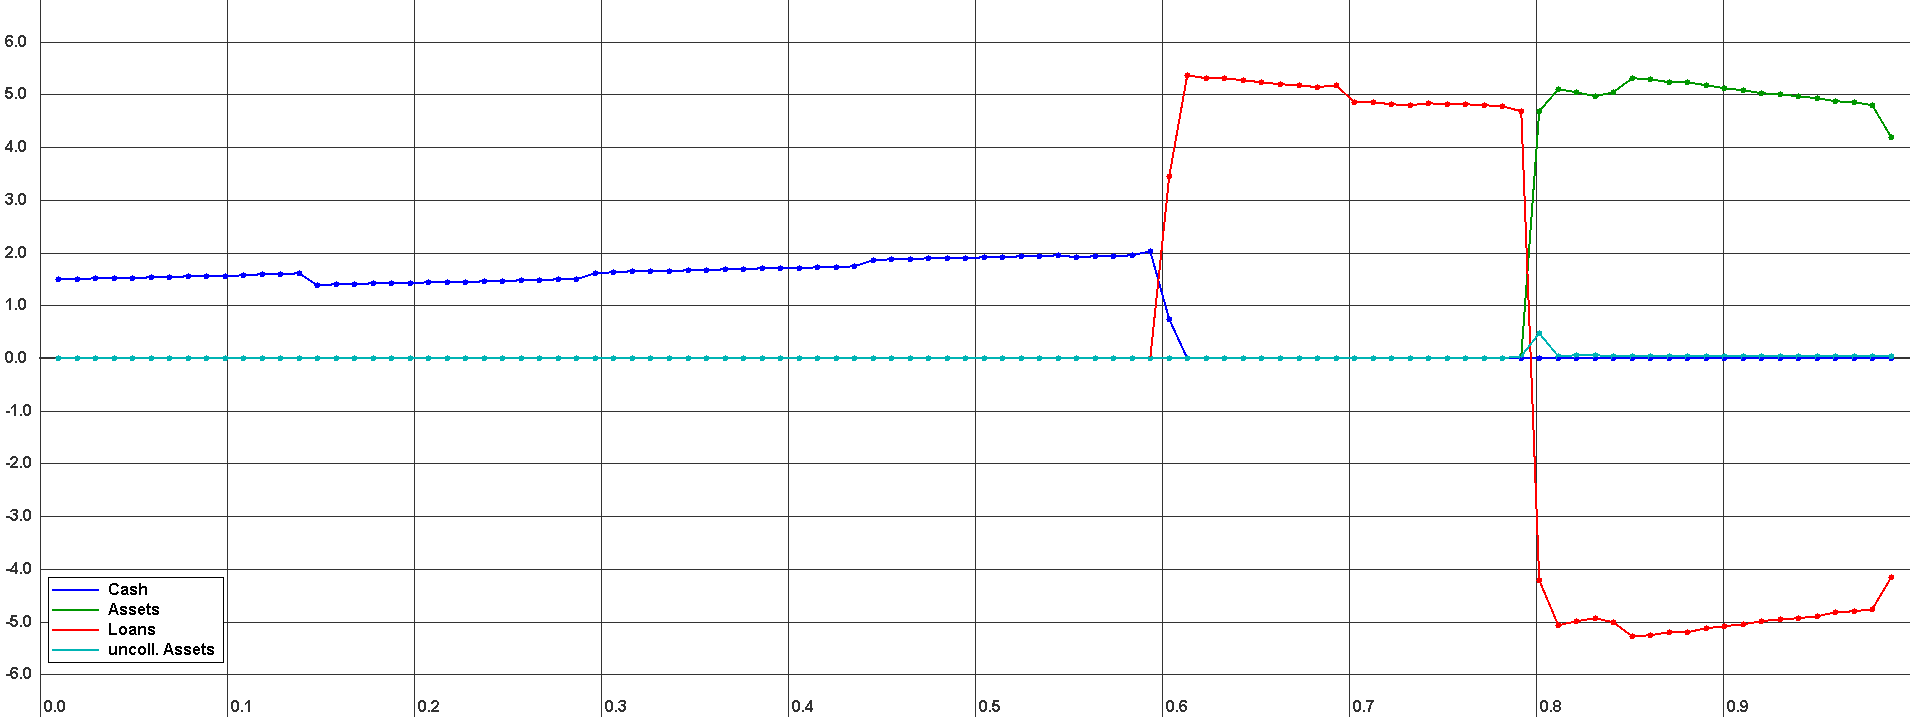
\includegraphics[width=1.0\textwidth, angle=0]{ASCENDINGCONNECTED_15RegSC_100_NOCOLLATERALMARKET_REPL.png}
	\caption{Ascending-Connected 15 regular short-cuts wealth-distribution after 50 replications}
	\label{fig1}
\end{figure}

\begin{table}[!htbp]
	\caption{Ascending-Connected 15 regular short-cuts equilibrium for 100 Agents}
	\centering
	\begin{tabular} { l c r }
		\hline
		Asset-Price & 0.705 (0.020) \\
		Loan-Price & 0.357 (0.018) \\
		i0 (Marginal Buyer) & 0.586 (0.023) \\
		i1 (Marginal Seller) & 0.802 (0.0) \\
		Pessimist Wealth & 1.649 (0.051) \\
		Medianist Wealth & 4.146 (0.101) \\
		Optimist Wealth & 4.997 (0.007) \\
		\hline
	\end{tabular}
\end{table} 

\begin{table}[!htbp]
	\caption{Ascending-Connected 15 regular short-cuts performance of 100 Agents}
	\centering
	\begin{tabular} { l c r }
		\hline
		Successful TX & 4373.28 (50.13) \\
		Total TX & 5502.52 (52.11) \\
		Failed TX & 1129.24 (19.2) \\
		\hline
	\end{tabular}
\end{table}

\subsection{Ascending-Connected 30 regular Short-cuts }
\begin{figure}[!htbp]
	\centering
  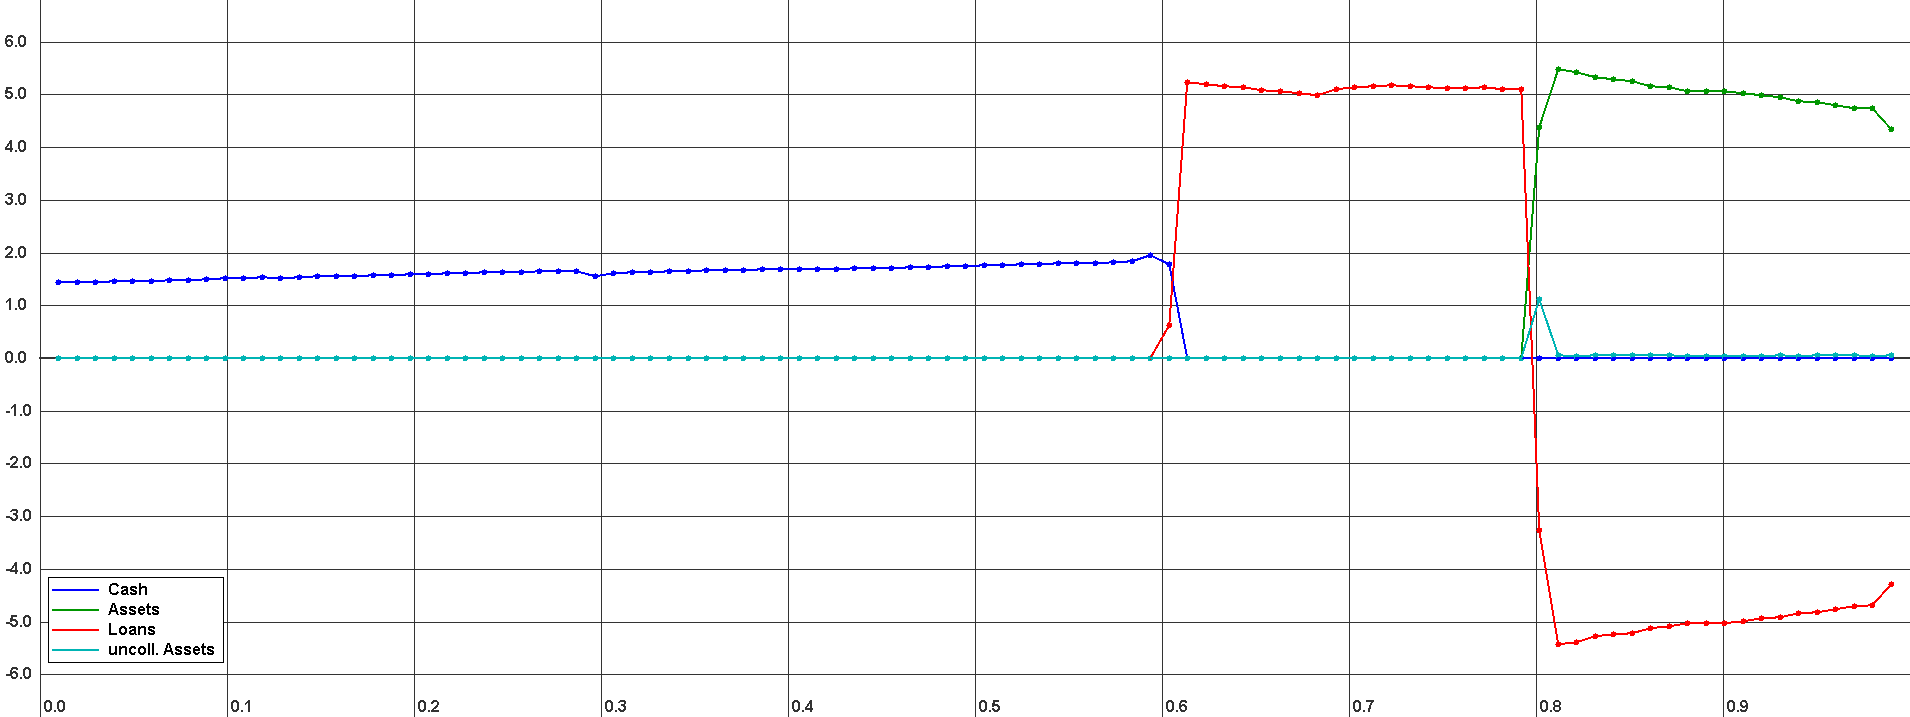
\includegraphics[width=1.0\textwidth, angle=0]{ASCENDINGCONNECTED_30RegSC_100_NOCOLLATERALMARKET_REPL.png}
	\caption{Ascending-Connected 30 regular short-cuts wealth-distribution after 50 replications}
	\label{fig1}
\end{figure}

\begin{table}[!htbp]
	\caption{Ascending-Connected 30 regular short-cuts equilibrium for 100 Agents}
	\centering
	\begin{tabular} { l c r }
		\hline
		Asset-Price & 0.710 (0.021) \\
		Loan-Price & 0.398 (0.008) \\
		i0 (Marginal Buyer) & 0.589 (0.021) \\
		i1 (Marginal Seller) & 0.802 (0.0) \\
		Pessimist Wealth & 1.479 (0.049) \\
		Medianist Wealth & 3.713 (0.125) \\
		Optimist Wealth & 5.0 (0.0) \\
		\hline
	\end{tabular}
\end{table} 

\begin{table}[!htbp]
	\caption{Ascending-Connected 30 regular short-cuts performance of 100 Agents}
	\centering
	\begin{tabular} { l c r }
		\hline
		Successful TX & 5427.02 (90.82) \\
		Total TX & 6566.06 (96.04) \\
		Failed TX & 1139.04 (27.74) \\
		\hline
	\end{tabular}
\end{table}

// TODO: Ascending-Connected 2 Short-Cuts
// TODO: Ascending-Connected 10 Full/regular Short-Cuts


\section{Deterministic Hub-Based Topologies} 
The Hub-Based Topologies fail to come even close to equilibrium due to reasons given in Chapter "Topologies and Hypothesis". This can be seen also very clearly in the visual results and thus no performance- and equilibrium-tables are listed as they would not make any sense.

\subsection{3-Hubs}
\begin{figure}[!htbp]
	\centering
  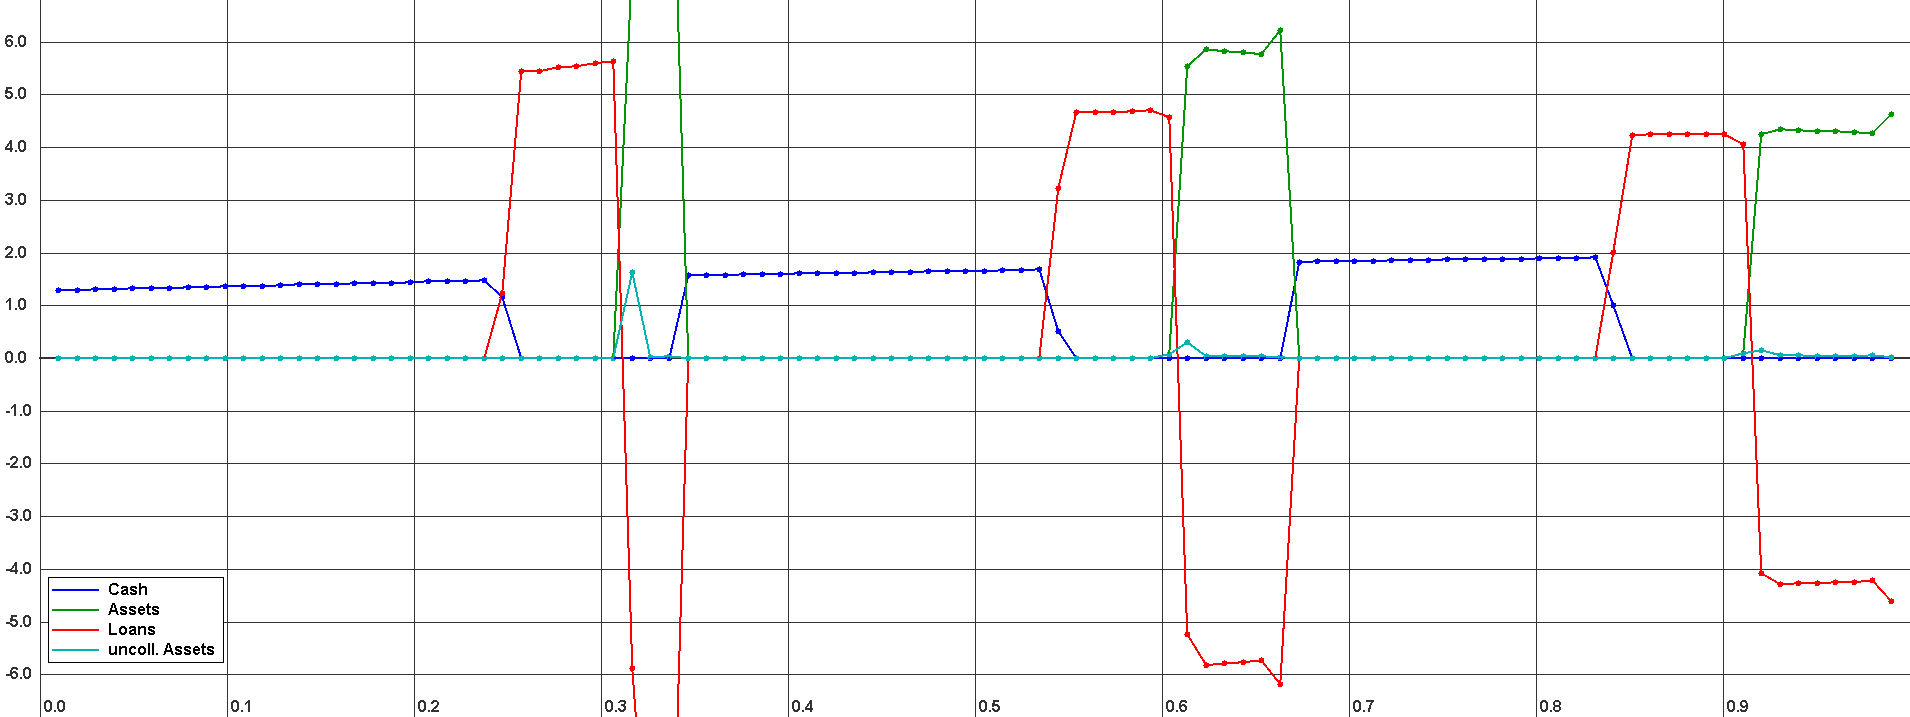
\includegraphics[width=1.0\textwidth, angle=0]{3HUBS_100_NOCOLLATERALMARKET_REPL.png}
	\caption{3-Hubs topology wealth-distribution after 50 replications}
	\label{fig1}
\end{figure}

\subsection{1-Median Hub}
\begin{figure}[!htbp]
	\centering
  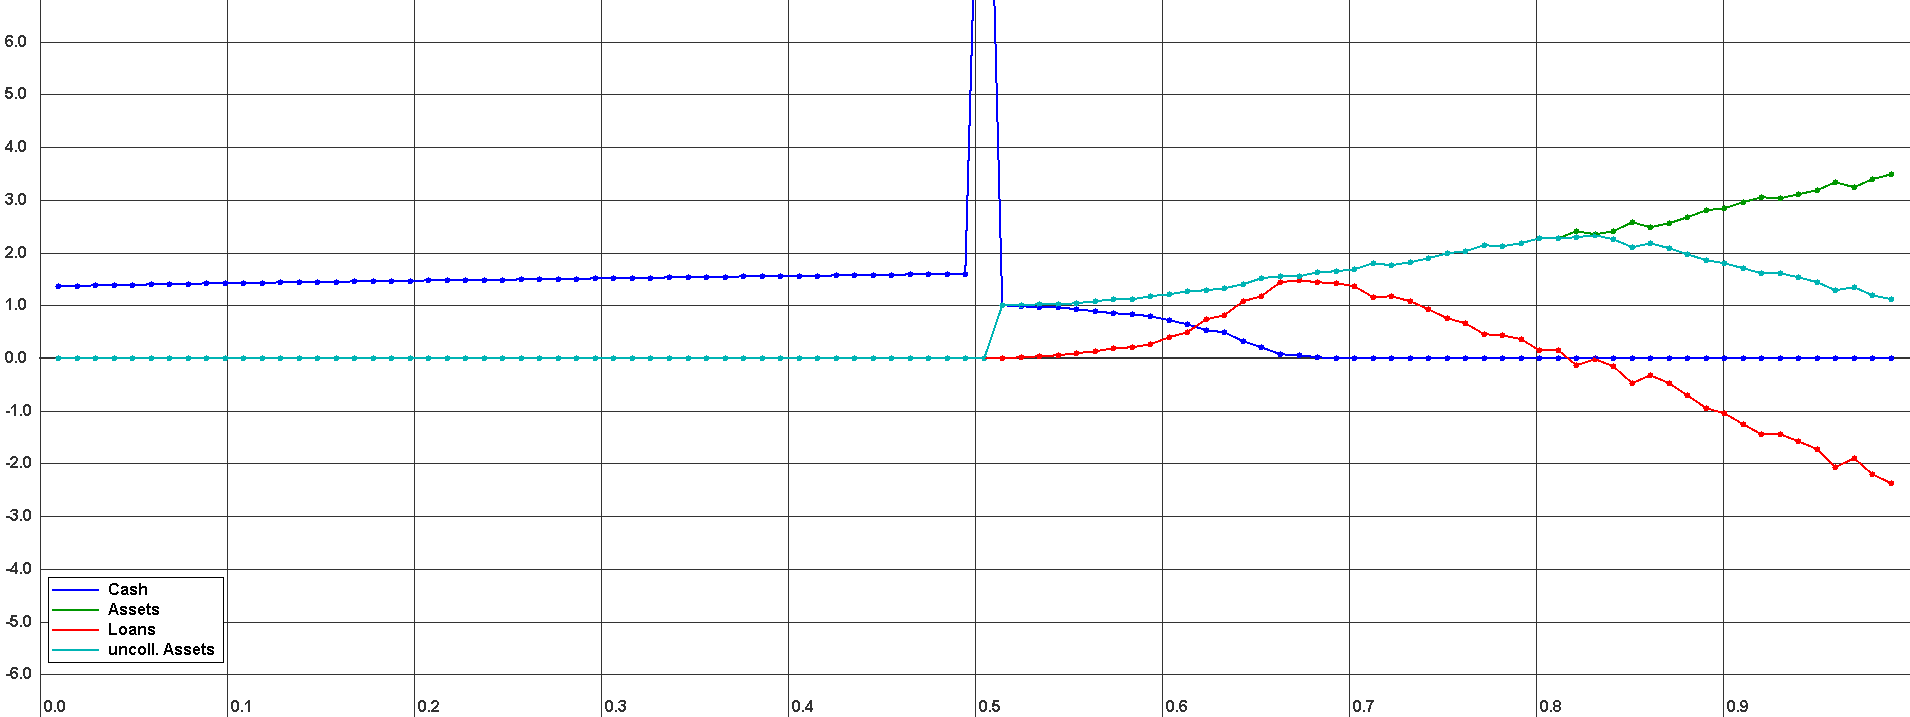
\includegraphics[width=1.0\textwidth, angle=0]{1MEDIANHUB_100_NOCOLLATERALMARKET_REPL.png}
	\caption{1 Median-Hub wealth-distribution after 50 replications}
	\label{fig1}
\end{figure}

\subsection{3-Median Hubs}
\begin{figure}[!htbp]
	\centering
  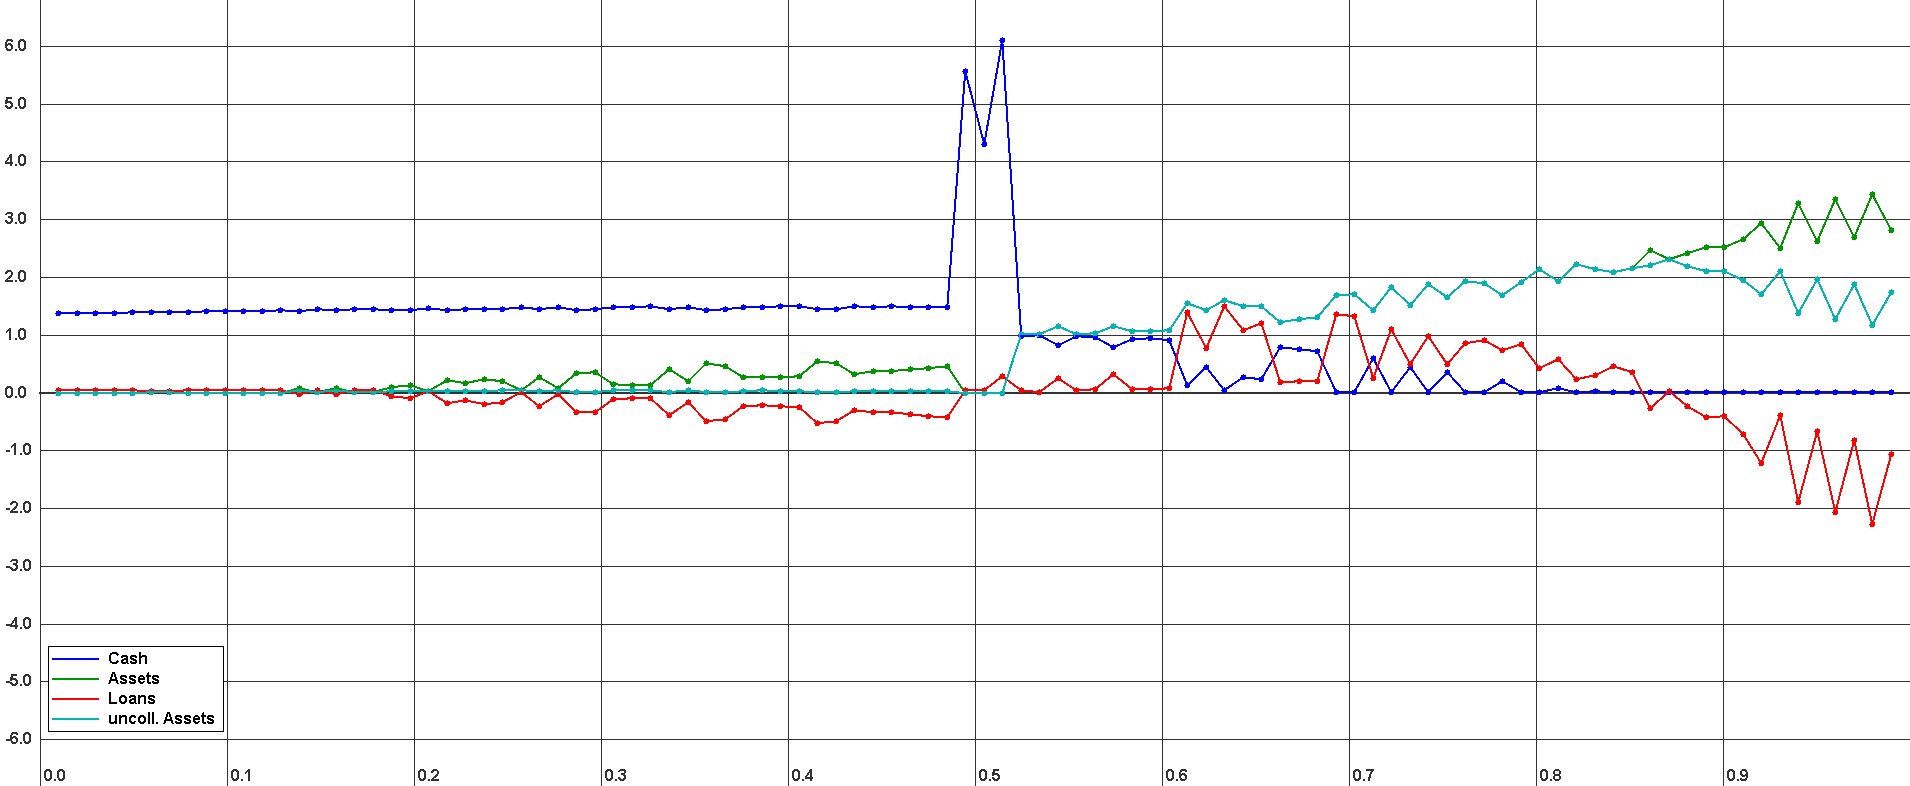
\includegraphics[width=1.0\textwidth, angle=0]{3MEDIANHUBS_100_NOCOLLATERALMARKET_REPL.png}
	\caption{3 Median-Hubs wealth-distribution after 50 replications}
	\label{fig1}
\end{figure}

\subsection{Maximum Hub}
\begin{figure}[!htbp]
	\centering
  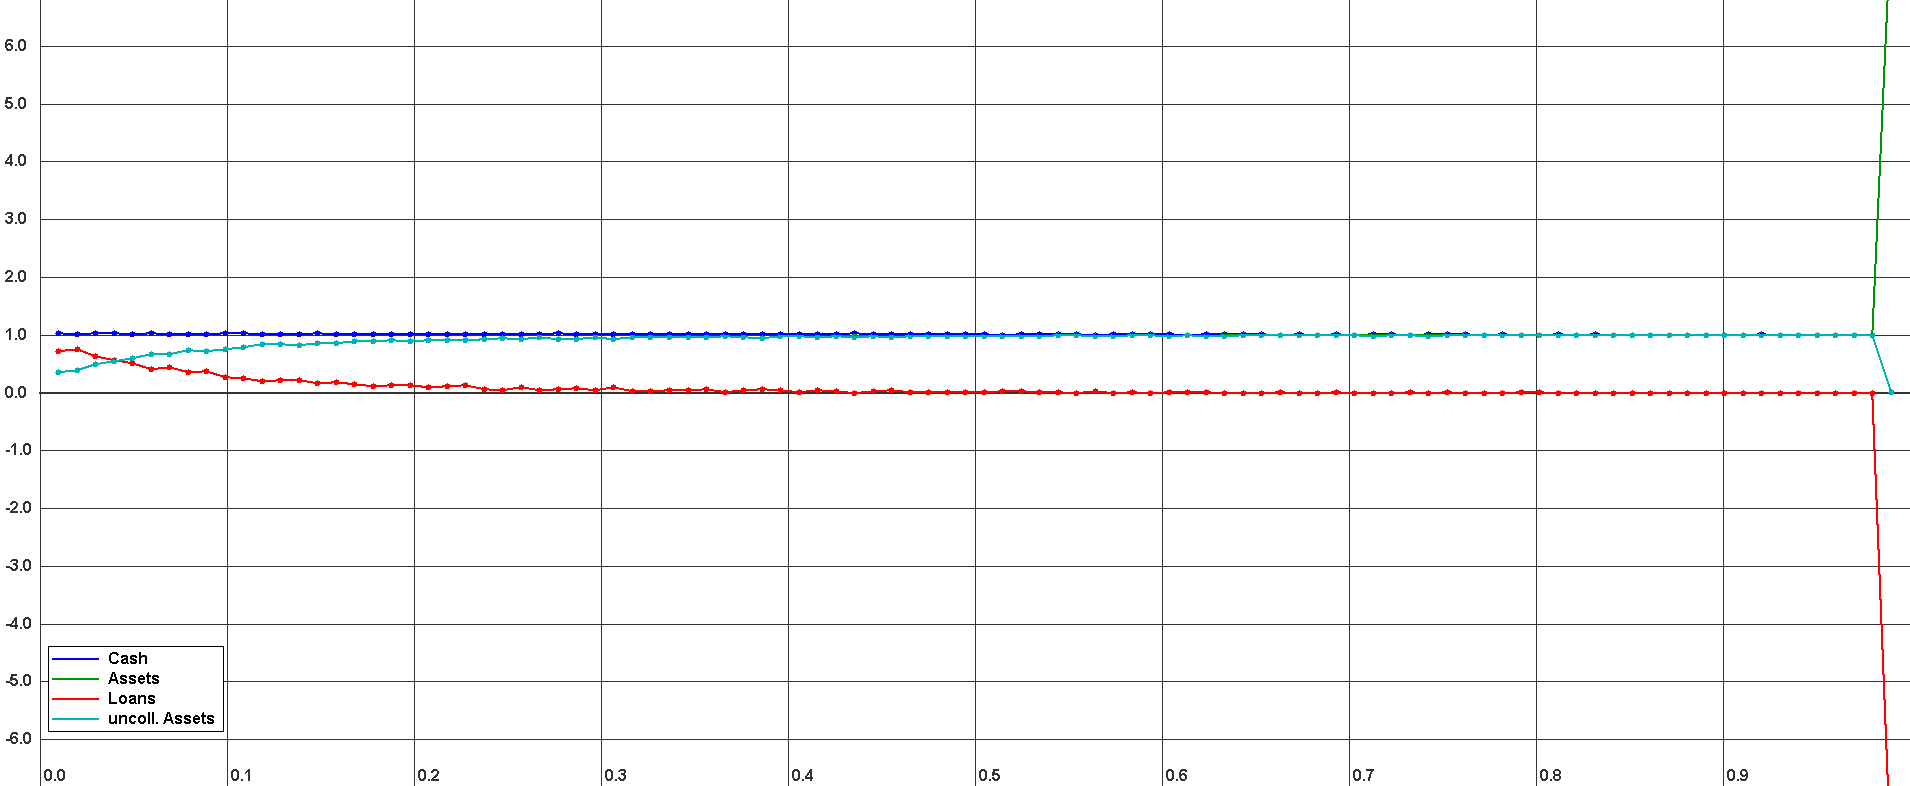
\includegraphics[width=1.0\textwidth, angle=0]{MAXIMUMHUB_100_NOCOLLATERALMARKET_REPL.png}
	\caption{Maximum-Hub wealth-distribution after 50 replications}
	\label{fig1}
\end{figure}

\section{Random-, Scale-Free and Small-World Topologies}
\subsection{Ascending-Connected random Short-cuts}
\subsection{Erdos-Renyi}
\subsection{Barbasi-Albert}
\subsection{Watts-Strogatz}

\end{document}
